
\documentclass[times,12pt,3p]{article}\usepackage[]{graphicx}\usepackage[]{color}
%% maxwidth is the original width if it is less than linewidth
%% otherwise use linewidth (to make sure the graphics do not exceed the margin)
\makeatletter
\def\maxwidth{ %
  \ifdim\Gin@nat@width>\linewidth
    \linewidth
  \else
    \Gin@nat@width
  \fi
}
\makeatother

\definecolor{fgcolor}{rgb}{0.345, 0.345, 0.345}
\newcommand{\hlnum}[1]{\textcolor[rgb]{0.686,0.059,0.569}{#1}}%
\newcommand{\hlstr}[1]{\textcolor[rgb]{0.192,0.494,0.8}{#1}}%
\newcommand{\hlcom}[1]{\textcolor[rgb]{0.678,0.584,0.686}{\textit{#1}}}%
\newcommand{\hlopt}[1]{\textcolor[rgb]{0,0,0}{#1}}%
\newcommand{\hlstd}[1]{\textcolor[rgb]{0.345,0.345,0.345}{#1}}%
\newcommand{\hlkwa}[1]{\textcolor[rgb]{0.161,0.373,0.58}{\textbf{#1}}}%
\newcommand{\hlkwb}[1]{\textcolor[rgb]{0.69,0.353,0.396}{#1}}%
\newcommand{\hlkwc}[1]{\textcolor[rgb]{0.333,0.667,0.333}{#1}}%
\newcommand{\hlkwd}[1]{\textcolor[rgb]{0.737,0.353,0.396}{\textbf{#1}}}%
\let\hlipl\hlkwb

\usepackage{framed}
\makeatletter
\newenvironment{kframe}{%
 \def\at@end@of@kframe{}%
 \ifinner\ifhmode%
  \def\at@end@of@kframe{\end{minipage}}%
  \begin{minipage}{\columnwidth}%
 \fi\fi%
 \def\FrameCommand##1{\hskip\@totalleftmargin \hskip-\fboxsep
 \colorbox{shadecolor}{##1}\hskip-\fboxsep
     % There is no \\@totalrightmargin, so:
     \hskip-\linewidth \hskip-\@totalleftmargin \hskip\columnwidth}%
 \MakeFramed {\advance\hsize-\width
   \@totalleftmargin\z@ \linewidth\hsize
   \@setminipage}}%
 {\par\unskip\endMakeFramed%
 \at@end@of@kframe}
\makeatother

\definecolor{shadecolor}{rgb}{.97, .97, .97}
\definecolor{messagecolor}{rgb}{0, 0, 0}
\definecolor{warningcolor}{rgb}{1, 0, 1}
\definecolor{errorcolor}{rgb}{1, 0, 0}
\newenvironment{knitrout}{}{} % an empty environment to be redefined in TeX

\usepackage{alltt}	

\usepackage{amsfonts,amsmath,amssymb}
\usepackage{pdfsync,subfig,multirow,tikz, pgfplots}
\usepackage{lmodern}
% \usepackage{hyperref}
\pgfplotsset{width=9cm, height=9cm, compat=1.3}
\newlength\longest
\linespread{1.3}
% \hyperlinking
\IfFileExists{upquote.sty}{\usepackage{upquote}}{}
\begin{document}
First we introduce the function GLC\_quadrature 

\begin{knitrout}
\definecolor{shadecolor}{rgb}{0.969, 0.969, 0.969}\color{fgcolor}\begin{kframe}
\begin{alltt}
\hlstd{GLC_quadrature} \hlkwb{<-} \hlkwa{function}\hlstd{(} \hlkwc{xmin}\hlstd{,} \hlkwc{xmax}\hlstd{,} \hlkwc{wanted_level}\hlstd{)}
\hlstd{\{}
\hlcom{# Generates an array of point corresponding to the Gauss-Lobatto-Tchebishev}
\hlcom{# quadrature comprised between user parameters xmin and xmax. The wanted}
\hlcom{# level for the quadrature is set by the wanted_level argument}
    \hlstd{x} \hlkwb{<-} \hlkwd{rep}\hlstd{(}\hlnum{0}\hlstd{,}\hlnum{2}\hlopt{^}\hlstd{(wanted_level}\hlopt{-}\hlnum{1}\hlstd{))}
    \hlstd{Points} \hlkwb{<-} \hlnum{2}\hlopt{^}\hlstd{wanted_level}
    \hlstd{index} \hlkwb{<-} \hlkwd{seq}\hlstd{(}\hlkwc{from}\hlstd{=}\hlnum{2}\hlstd{,} \hlkwc{to}\hlstd{=Points,}\hlkwc{by}\hlstd{=}\hlnum{2}\hlstd{)}
    \hlstd{aux} \hlkwb{<-} \hlopt{-}\hlkwd{cos}\hlstd{(pi}\hlopt{*}\hlstd{(index}\hlopt{-}\hlnum{1}\hlstd{)}\hlopt{/}\hlstd{Points)}
    \hlstd{x}\hlkwb{<-} \hlstd{xmin} \hlopt{+} \hlstd{(xmax}\hlopt{-}\hlstd{xmin)}\hlopt{*}\hlstd{(aux}\hlopt{+}\hlnum{1}\hlstd{)}\hlopt{/}\hlnum{2}
    \hlkwd{return}\hlstd{(x)}
\hlstd{\}}
\end{alltt}
\end{kframe}
\end{knitrout}

We use a library for the scatterplots and to write excel files:

\begin{knitrout}
\definecolor{shadecolor}{rgb}{0.969, 0.969, 0.969}\color{fgcolor}\begin{kframe}
\begin{alltt}
\hlcom{#we use the library('scatterplot3d') and library('WriteXLS')}
\hlkwd{library}\hlstd{(}\hlstr{'scatterplot3d'}\hlstd{)}
\hlkwd{library}\hlstd{(}\hlstr{'WriteXLS'}\hlstd{)}
\end{alltt}
\end{kframe}
\end{knitrout}

Next we give maximal level for Gauss Lobatto Chebyshev quadratures:

\begin{knitrout}
\definecolor{shadecolor}{rgb}{0.969, 0.969, 0.969}\color{fgcolor}\begin{kframe}
\begin{alltt}
\hlcom{#value of the maximal level for Gauss Lobatto Chebyshev quadratures}
\hlstd{lvlmax} \hlkwb{<-} \hlnum{9}
\hlcom{#min/max values for parameter 1 }
\hlstd{xmin_param_1} \hlkwb{<-} \hlnum{0}
\hlstd{xmax_param_1} \hlkwb{<-} \hlnum{10}
\hlcom{#min/max values for parameter 2}
\hlstd{xmin_param_2} \hlkwb{<-} \hlnum{10}
\hlstd{xmax_param_2} \hlkwb{<-}\hlnum{20}
\hlcom{#min/max values for parameter 3}
\hlstd{xmin_param_3} \hlkwb{<-} \hlopt{-}\hlnum{10}
\hlstd{xmax_param_3} \hlkwb{<-} \hlnum{5}
\hlcom{# !!! TO CLOSE ONE DIMENSION/PARAMETER, JUST PUT THE SAME VALUE FOR XMIN AND}
\hlcom{#XMAX !!!}
\end{alltt}
\end{kframe}
\end{knitrout}

Now, we proceed to execute the rest of the R-code:

\begin{knitrout}
\definecolor{shadecolor}{rgb}{0.969, 0.969, 0.969}\color{fgcolor}
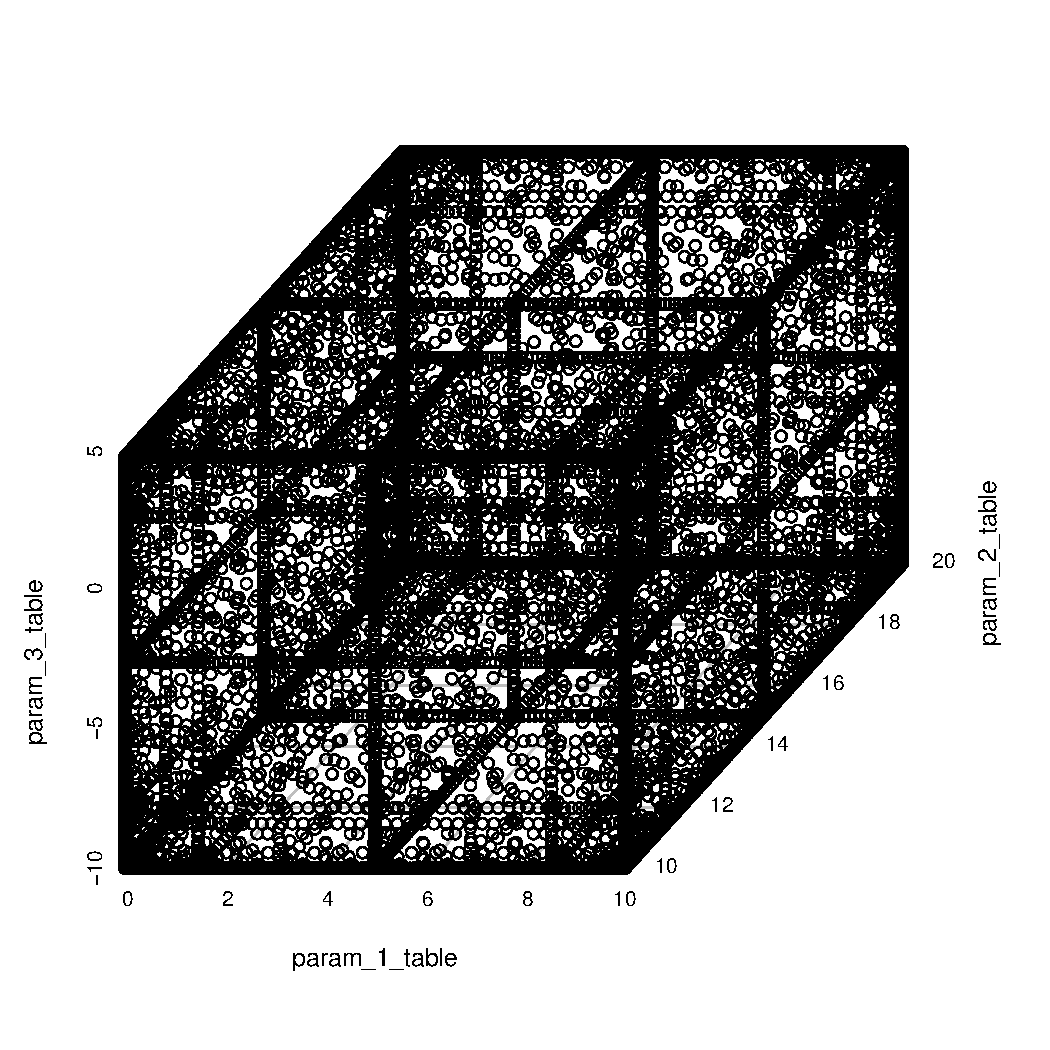
\includegraphics[width=\maxwidth]{figure/unnamed-chunk-2-1} 

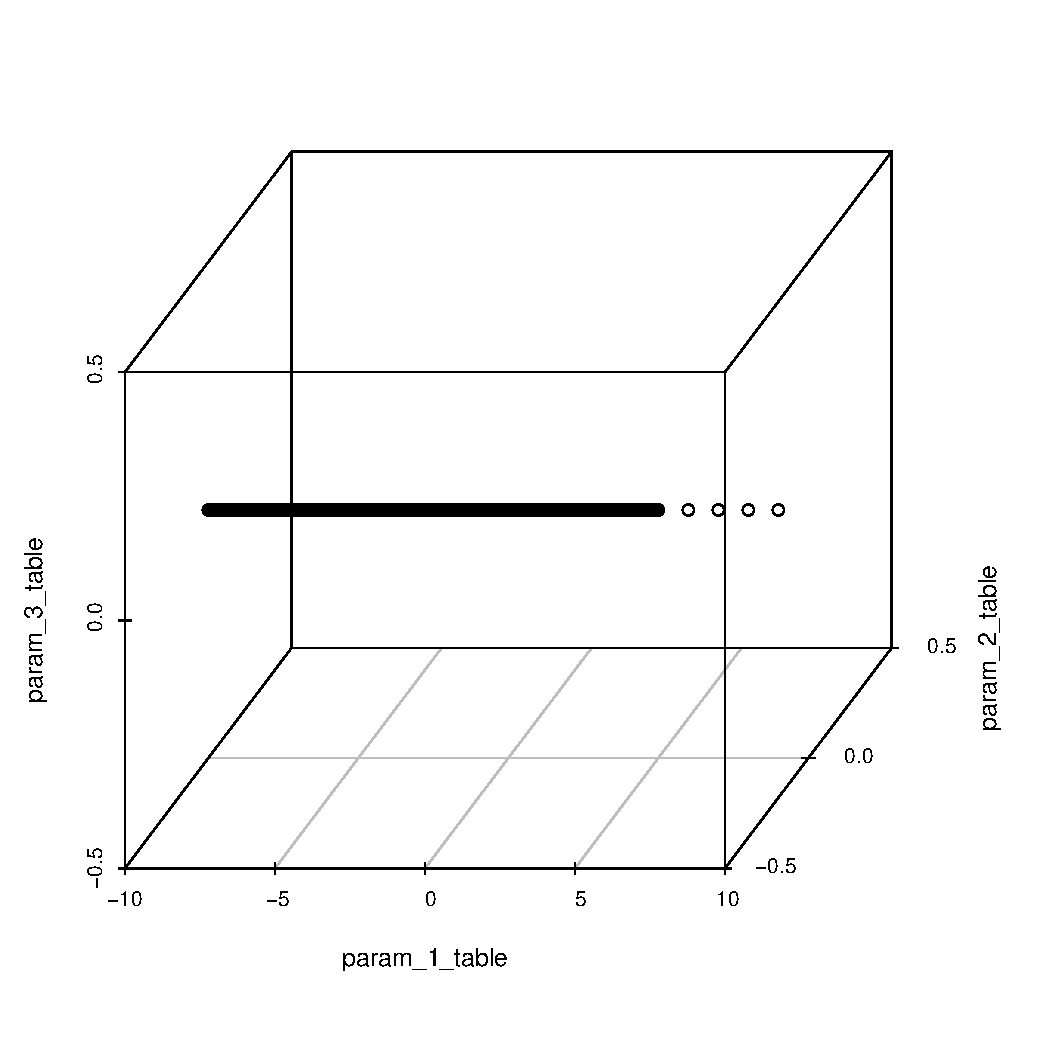
\includegraphics[width=\maxwidth]{figure/unnamed-chunk-2-2} 

\end{knitrout}
\end{document}
